\documentclass[tikz,class=article]{standalone}


\begin{document}

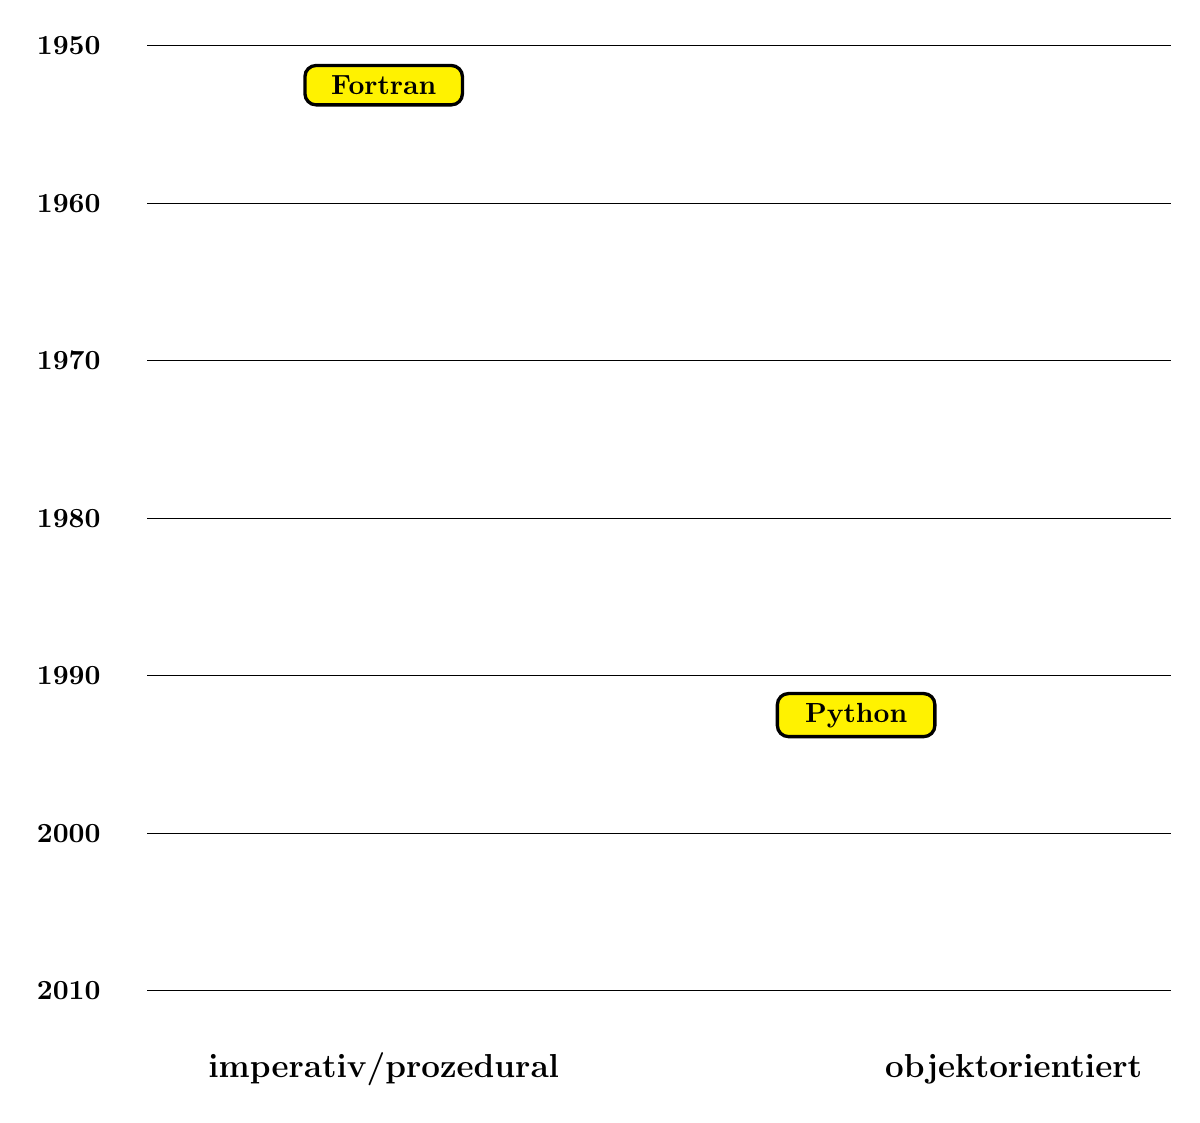
\begin{tikzpicture}
[
    mybox/.style={rectangle,rounded corners,xshift=1cm,yshift=1cm,minimum width=20mm, minimum height=5mm},
    lang/.style={mybox,black,align=center,draw=black,fill=yellow,very thick,font=\bfseries},
]
 
\node at (5,-1) {\bfseries\large imperativ/prozedural};
\node at (13,-1) {\bfseries\large objektorientiert};
 
\node at (1,12) {\textbf{1950}};
\node at (1,10) {\textbf{1960}};
\node at (1,8) {\textbf{1970}};
\node at (1,6) {\textbf{1980}};
\node at (1,4) {\textbf{1990}};
\node at (1,2) {\textbf{2000}};
\node at (1,0) {\textbf{2010}};
 
\draw (2,0) -- (15,0);
\draw (2,2) -- (15,2);
\draw (2,4) -- (15,4);
\draw (2,6) -- (15,6);
\draw (2,8) -- (15,8);
\draw (2,10) -- (15,10);
\draw (2,12) -- (15,12);
 
\node at (10,2.5) [lang] {Python};
\node at (4,10.5) [lang] {Fortran};
\end{tikzpicture}

\end{document}